\section{Results}

\subsection{Hypothesis Testing}

\subsubsection{Hypothesis 1: Education and Employment Status}

\begin{table}[H]
    \caption{Chi-Square Test Results}
    \label{tab:chi_square_results}
    \begin{minipage}{\columnwidth}
        \centering
        \begin{tabular}{lll}
\toprule
 & $\chi^2$ & $p$ \\
\midrule
Value & 905.29 & 0.00 \\
\bottomrule
\end{tabular}

    \end{minipage}
\end{table}

\begin{table}[H]
    \centering
    \scriptsize
    \caption{Logistic regression results}
    \begin{minipage}{\columnwidth}
        \begin{center}
\begin{tabular}{lclc}
\toprule
\textbf{Dep. Variable:}      & employ\_Status2  & \textbf{  No. Observations:  } &    28853    \\
\textbf{Model:}              &      Logit       & \textbf{  Df Residuals:      } &    28851    \\
\textbf{Method:}             &       MLE        & \textbf{  Df Model:          } &        1    \\
\textbf{Date:}               & Mon, 30 Sep 2024 & \textbf{  Pseudo R-squ.:     } &  0.01560    \\
\textbf{Time:}               &     15:55:34     & \textbf{  Log-Likelihood:    } &   -18330.   \\
\textbf{converged:}          &       True       & \textbf{  LL-Null:           } &   -18621.   \\
\textbf{Covariance Type:}    &    nonrobust     & \textbf{  LLR p-value:       } & 2.302e-128  \\
\bottomrule
\end{tabular}
\begin{tabular}{lcccccc}
                             & \textbf{coef} & \textbf{std err} & \textbf{z} & \textbf{P$> |$z$|$} & \textbf{[0.025} & \textbf{0.975]}  \\
\midrule
\textbf{const}               &       0.4097  &        0.046     &     8.951  &         0.000        &        0.320    &        0.499     \\
\textbf{education\_category} &      -0.3346  &        0.014     &   -23.366  &         0.000        &       -0.363    &       -0.307     \\
\bottomrule
\end{tabular}
%\caption{Logit Regression Results}
\end{center}
    \end{minipage}
\end{table}

\begin{figure}[H]
    \centering
    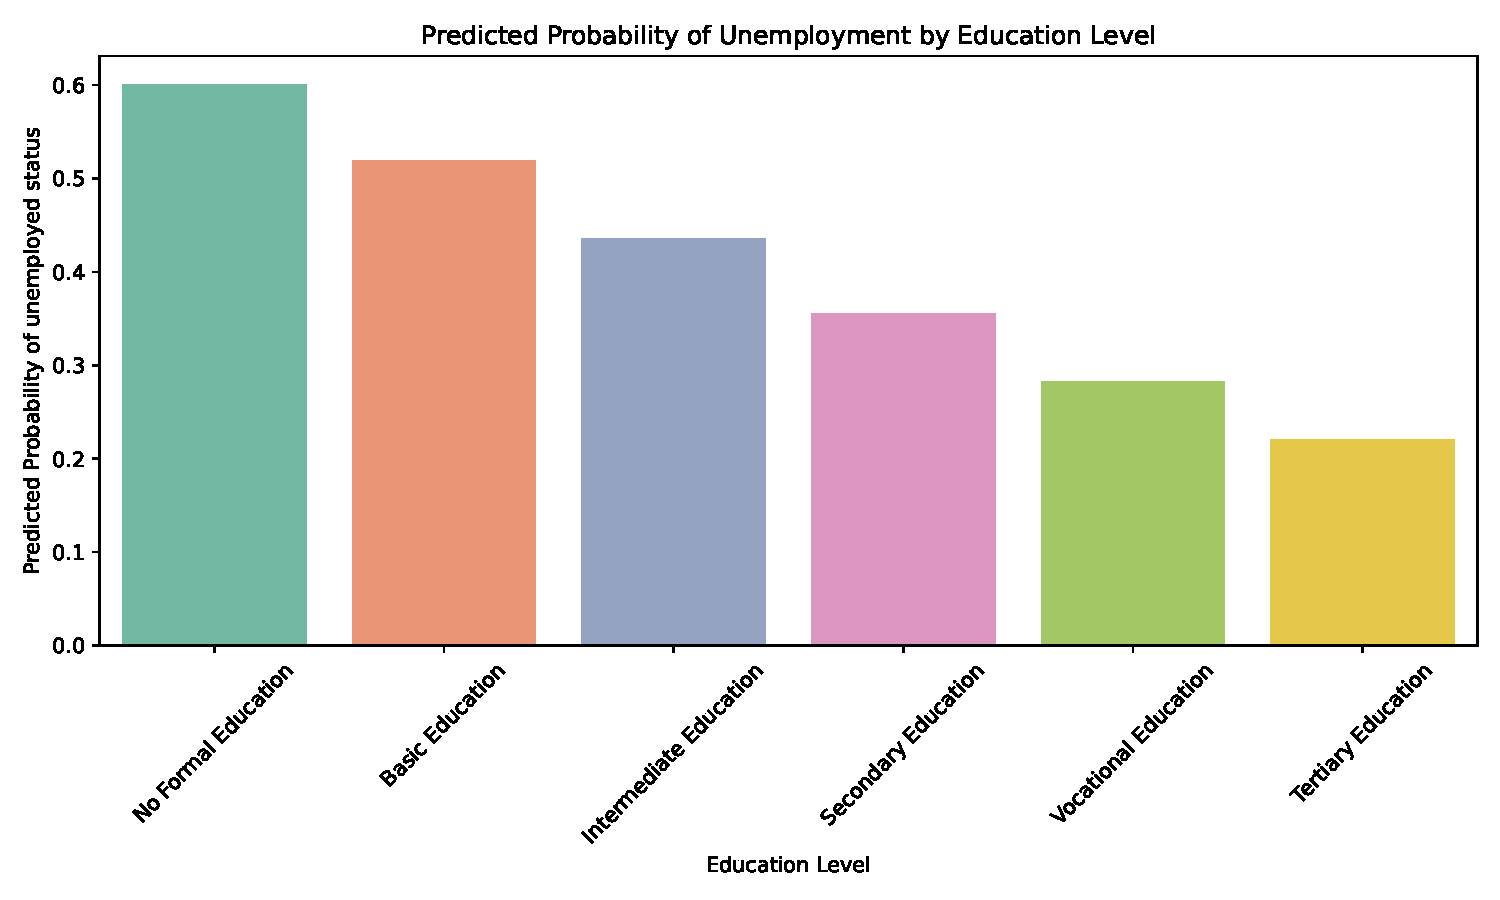
\includegraphics[width=\columnwidth]{images/hyp_1_log_pred.pdf} % Adjust the path accordingly
    \caption{Caption for the pdf image.}
    \label{fig:predicted unemployment for highest academic level}
\end{figure}

\begin{figure}[H]
    \centering
    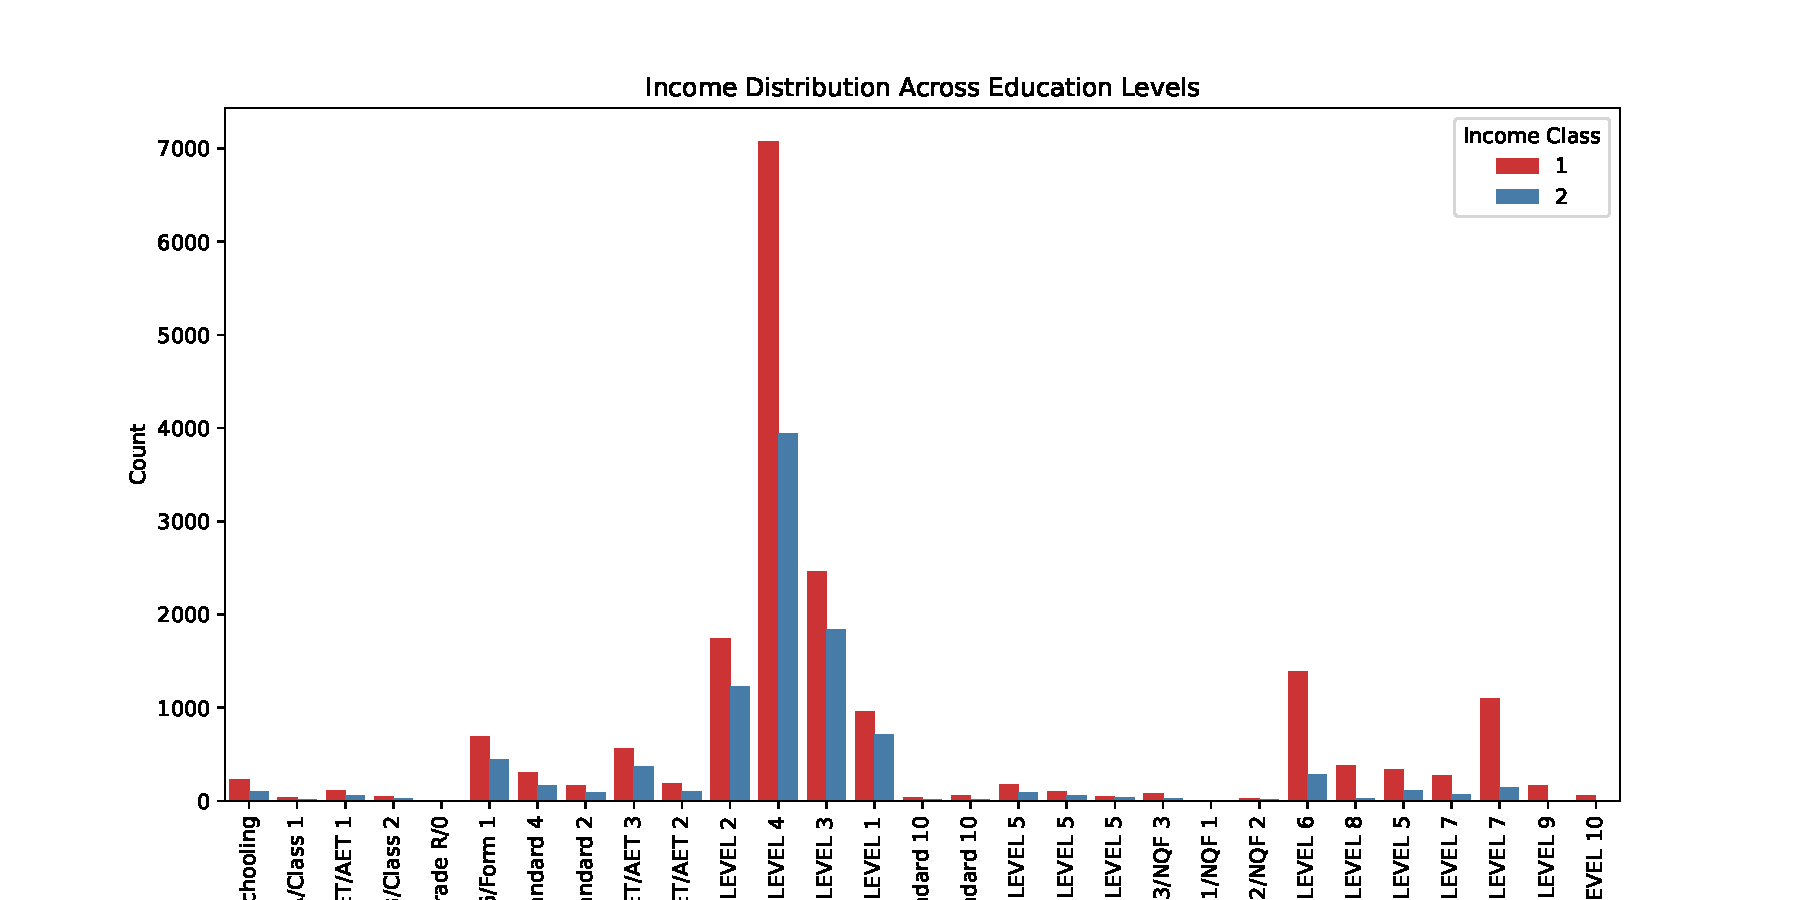
\includegraphics[width=\columnwidth]{images/hyp_1_income_dist.pdf} % Adjust the path accordingly
    \caption{Caption for the pdf image.}
    \label{fig:unemployment distribution for unemployment highest academic level}
\end{figure}

The chi-square test for independence showed a significant relationship between education level and employment status ($\chi^2 = X.XX$, $p < 0.05$). This suggests that higher levels of education are associated with higher employment rates.

\subsubsection{Hypothesis 2: Education and Salary}

\begin{figure}[H]
    \centering
    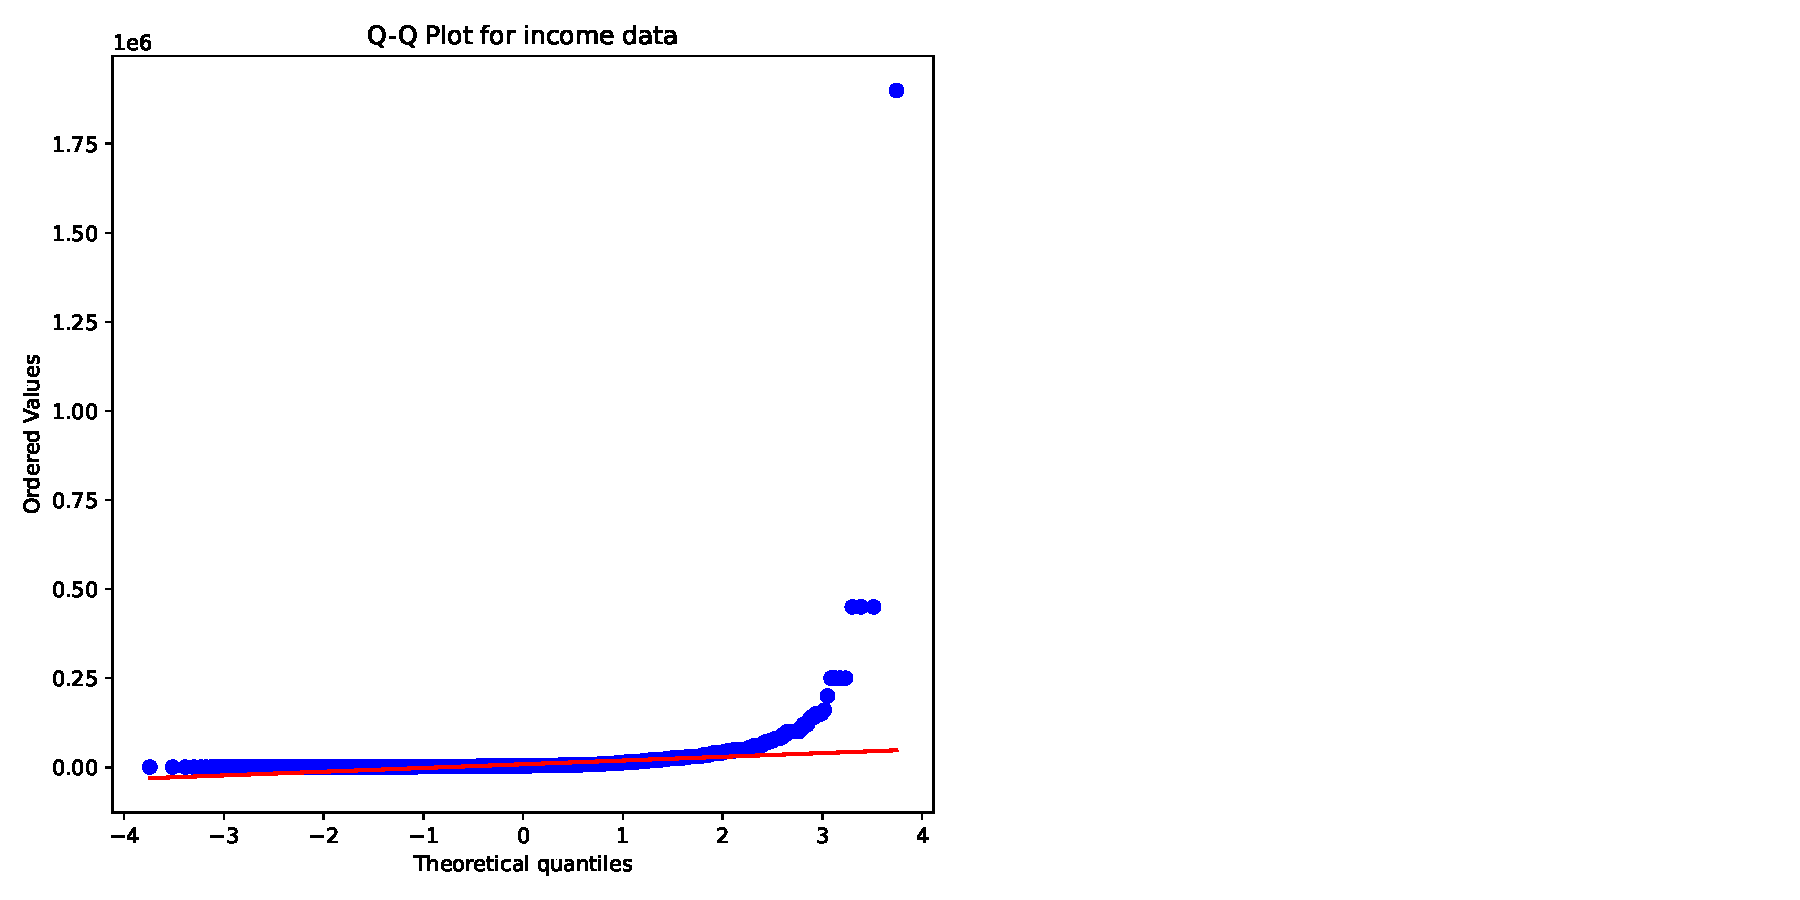
\includegraphics[width=\columnwidth]{images/hyp_2_norm_dist_income data.pdf} % Adjust the path accordingly
    \caption{Caption for the pdf image.}
    \label{fig:Independence test for anova test}
\end{figure}

\begin{table}[H]
    \centering
    \caption{Levene independence test results}
    \label{tab:Levene test results}
    \begin{minipage}{\columnwidth}
        \begin{tabular}{rrrrr}
\toprule
df & sum\_sq & mean\_sq & F & PR(>F) \\
\midrule
5.000 & 271399165518.753 & 54279833103.751 & 79.258 & 0.000 \\
7590.000 & 5198036057205.649 & 684853235.468 & NaN & NaN \\
\bottomrule
\end{tabular}

    \end{minipage}
\end{table}

\begin{table}[H]
    \centering
    \scriptsize
    \caption{Tukey test results}
    \label{tab:tukey test results}
    \begin{minipage}{\columnwidth}
        \centering
        \begin{tabular}{lrrrrrrr}
\toprule
 & group1 & group2 & meandiff & p-adj & lower & upper & reject \\
\midrule
0 & 0.0000 & 1.0000 & 146.5434 & 1.0000 & -8890.4647 & 9183.5515 & False \\
1 & 0.0000 & 2.0000 & 716.2572 & 0.9996 & -5822.8625 & 7255.3770 & False \\
2 & 0.0000 & 3.0000 & 4063.5954 & 0.4301 & -2179.2058 & 10306.3967 & False \\
3 & 0.0000 & 4.0000 & 9090.1826 & 0.0215 & 818.1259 & 17362.2394 & True \\
4 & 0.0000 & 5.0000 & 20251.3632 & 0.0000 & 13676.4532 & 26826.2732 & True \\
5 & 1.0000 & 2.0000 & 569.7139 & 0.9999 & -6410.3448 & 7549.7726 & False \\
6 & 1.0000 & 3.0000 & 3917.0521 & 0.5547 & -2786.2083 & 10620.3125 & False \\
7 & 1.0000 & 4.0000 & 8943.6393 & 0.0369 & 318.7882 & 17568.4903 & True \\
8 & 1.0000 & 5.0000 & 20104.8198 & 0.0000 & 13091.2206 & 27118.4191 & True \\
9 & 2.0000 & 3.0000 & 3347.3382 & 0.0014 & 892.4917 & 5802.1847 & True \\
10 & 2.0000 & 4.0000 & 8373.9254 & 0.0009 & 2417.3637 & 14330.4870 & True \\
11 & 2.0000 & 5.0000 & 19535.1059 & 0.0000 & 16328.3715 & 22741.8404 & True \\
12 & 3.0000 & 4.0000 & 5026.5872 & 0.1114 & -603.0760 & 10656.2504 & False \\
13 & 3.0000 & 5.0000 & 16187.7677 & 0.0000 & 13639.1158 & 18736.4197 & True \\
14 & 4.0000 & 5.0000 & 11161.1806 & 0.0000 & 5165.3502 & 17157.0109 & True \\
\bottomrule
\end{tabular}

    \end{minipage}
\end{table}

\subsubsection{Hypothesis 3: Age and Salary}

\begin{table}[H]
    \centering
    \caption{Pearson correlation test results}
    \label{tab:pearson correlation test results}
    \begin{minipage}{\columnwidth}
        \begin{tabular}{lll}
\toprule
 & Pearson correlation statistic & $p$ \\
\midrule
Value & 0.06 & 0.00 \\
\bottomrule
\end{tabular}

    \end{minipage}
\end{table}

\begin{table}[H]
    \centering
    \scriptsize
    \caption{Robust OLS regresion results}
    \label{tab:robust ols regression test results}
    \begin{minipage}{\columnwidth}
        \centering
        \begin{center}
\begin{tabular}{lclc}
\toprule
\textbf{Dep. Variable:}      & employ\_Status2  & \textbf{  No. Observations:  } &    28853    \\
\textbf{Model:}              &      Logit       & \textbf{  Df Residuals:      } &    28851    \\
\textbf{Method:}             &       MLE        & \textbf{  Df Model:          } &        1    \\
\textbf{Date:}               & Mon, 30 Sep 2024 & \textbf{  Pseudo R-squ.:     } &  0.01560    \\
\textbf{Time:}               &     15:49:38     & \textbf{  Log-Likelihood:    } &   -18330.   \\
\textbf{converged:}          &       True       & \textbf{  LL-Null:           } &   -18621.   \\
\textbf{Covariance Type:}    &    nonrobust     & \textbf{  LLR p-value:       } & 2.302e-128  \\
\bottomrule
\end{tabular}
\begin{tabular}{lcccccc}
                             & \textbf{coef} & \textbf{std err} & \textbf{z} & \textbf{P$> |$z$|$} & \textbf{[0.025} & \textbf{0.975]}  \\
\midrule
\textbf{const}               &       0.4097  &        0.046     &     8.951  &         0.000        &        0.320    &        0.499     \\
\textbf{education\_category} &      -0.3346  &        0.014     &   -23.366  &         0.000        &       -0.363    &       -0.307     \\
\bottomrule
\end{tabular}
%\caption{Logit Regression Results}
\end{center}
    \end{minipage}
\end{table}

\begin{figure}[H]
    \centering
    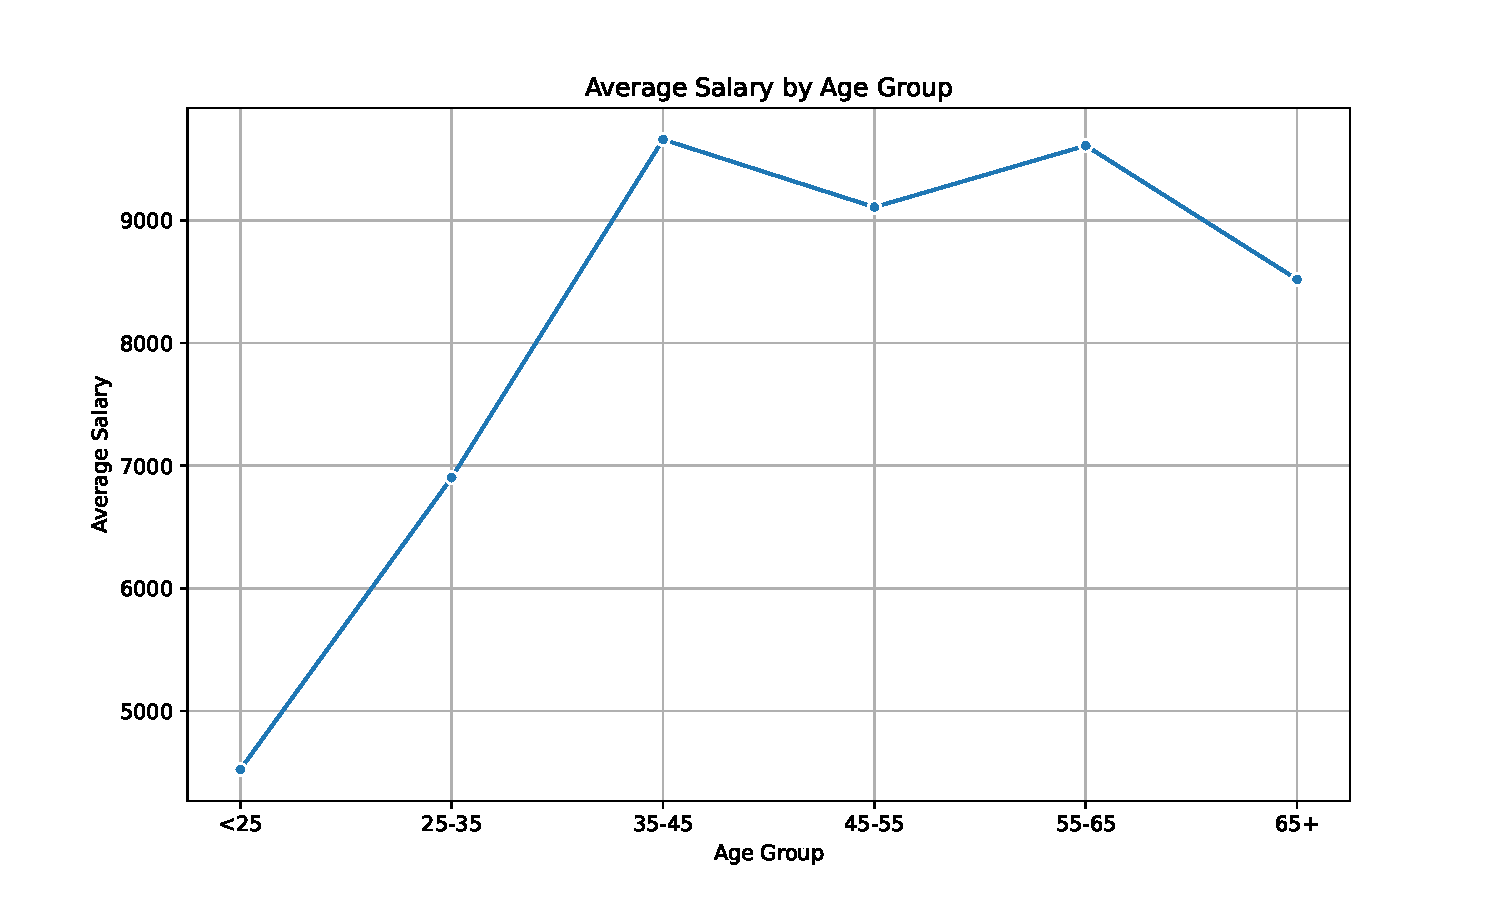
\includegraphics[width=\columnwidth]{images/hyp_3_average_salary.pdf} % Adjust the path accordingly
    \caption{Average salary vs age}
    \label{fig:Average salary by age scatter plot}
\end{figure}

\begin{figure}[H]
    \centering
    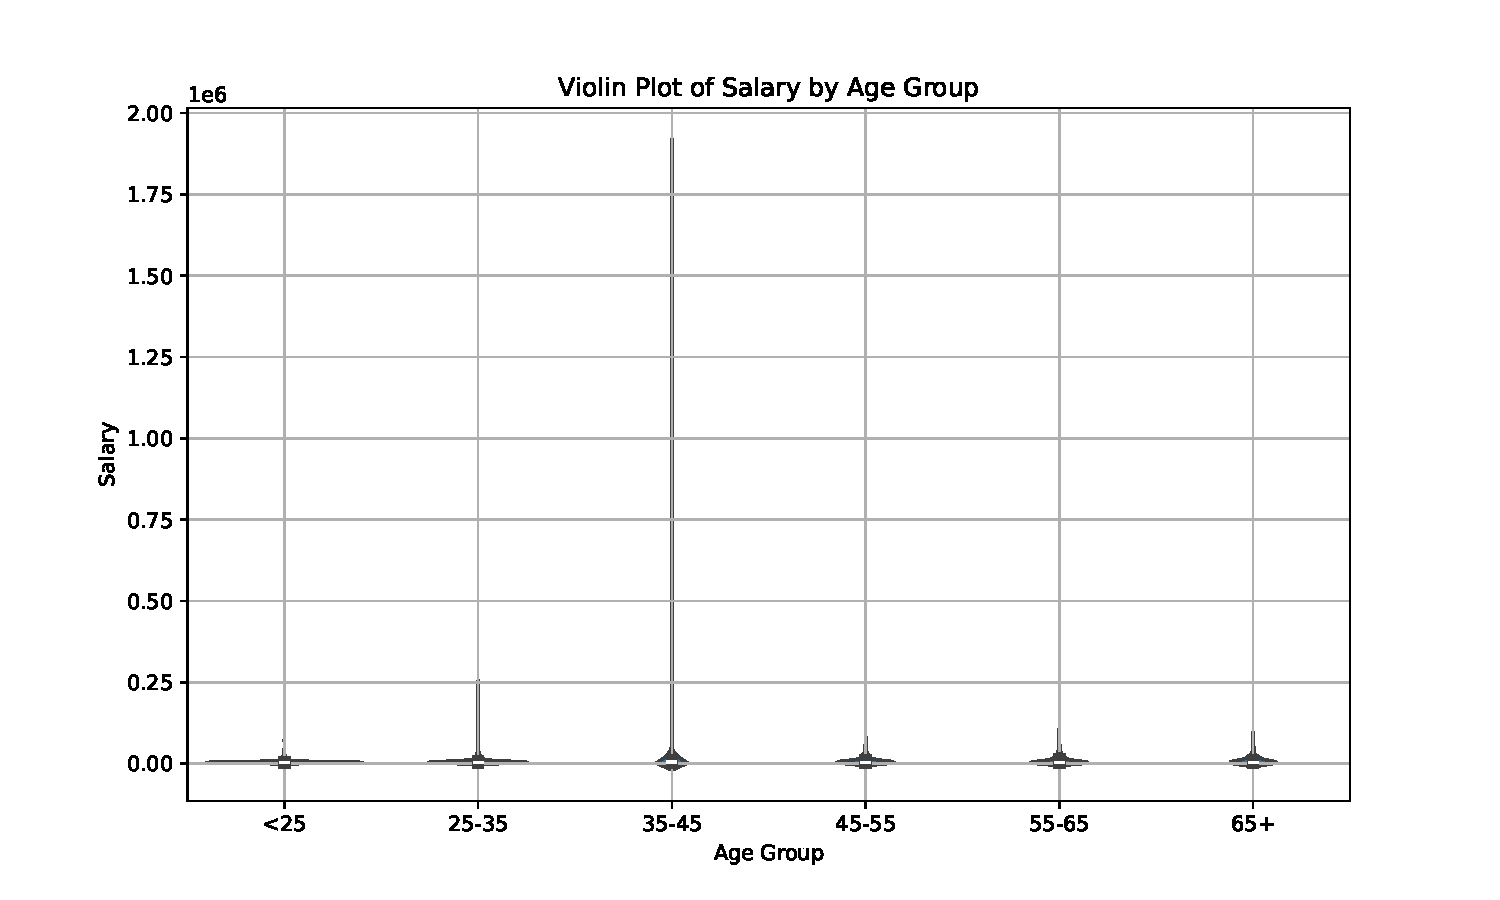
\includegraphics[width=\columnwidth]{images/hyp3_salary_by_age_violin.pdf} % Adjust the path accordingly
    \caption{Violion plot of salary by age group}
    \label{fig:violion plot of salary by age group}
\end{figure}

\begin{figure}[H]
    \centering
    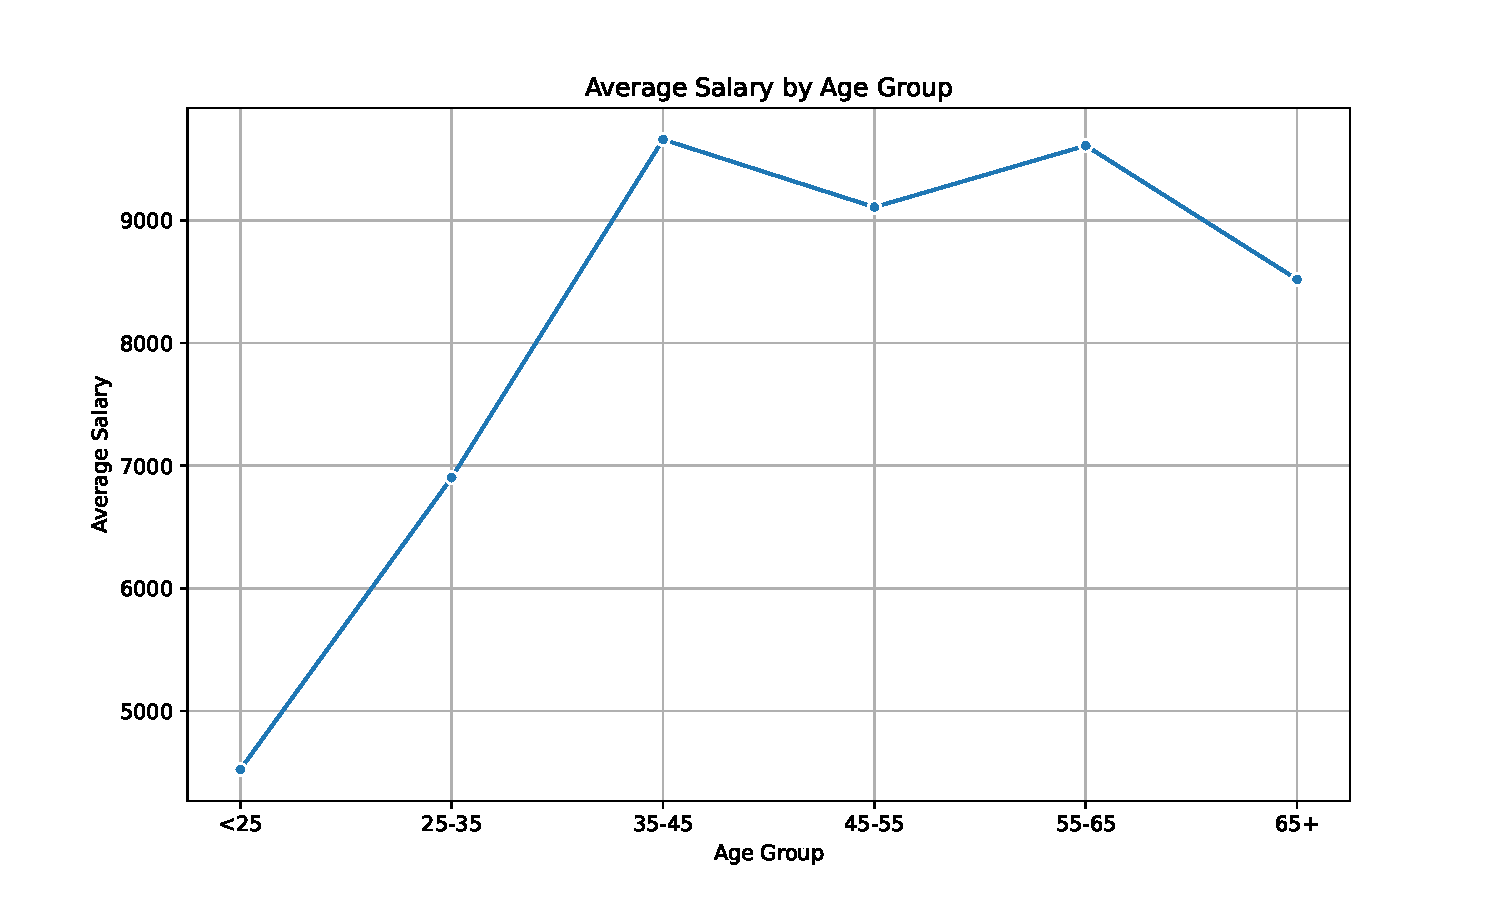
\includegraphics[width=\columnwidth]{images/hyp_3_average_salary.pdf} % Adjust the path accordingly
    \caption{Average salary per age group}
    \label{fig:average salary per age group}
\end{figure}

\begin{figure}[H]
    \centering
    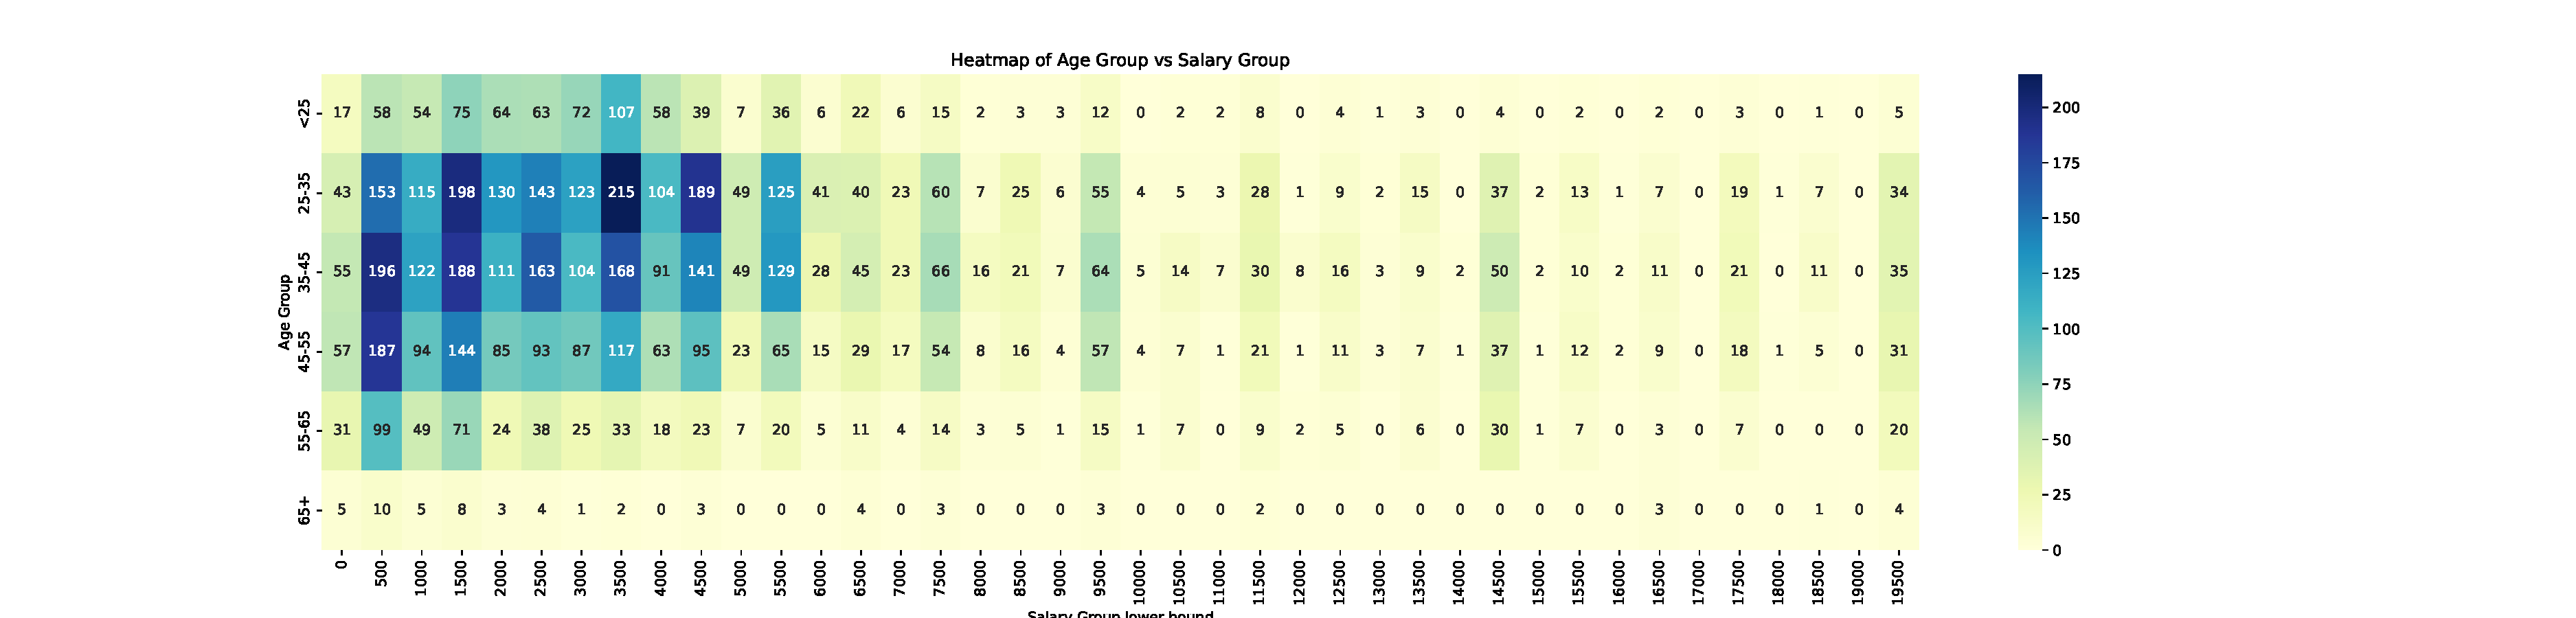
\includegraphics[width=\columnwidth]{images/hyp_3_heat_map.pdf} % Adjust the path accordingly
    \caption{Heat map of salary distribution by age group}
    \label{fig:salary distribution heat map}
\end{figure}

\begin{figure}[H]
    \centering
    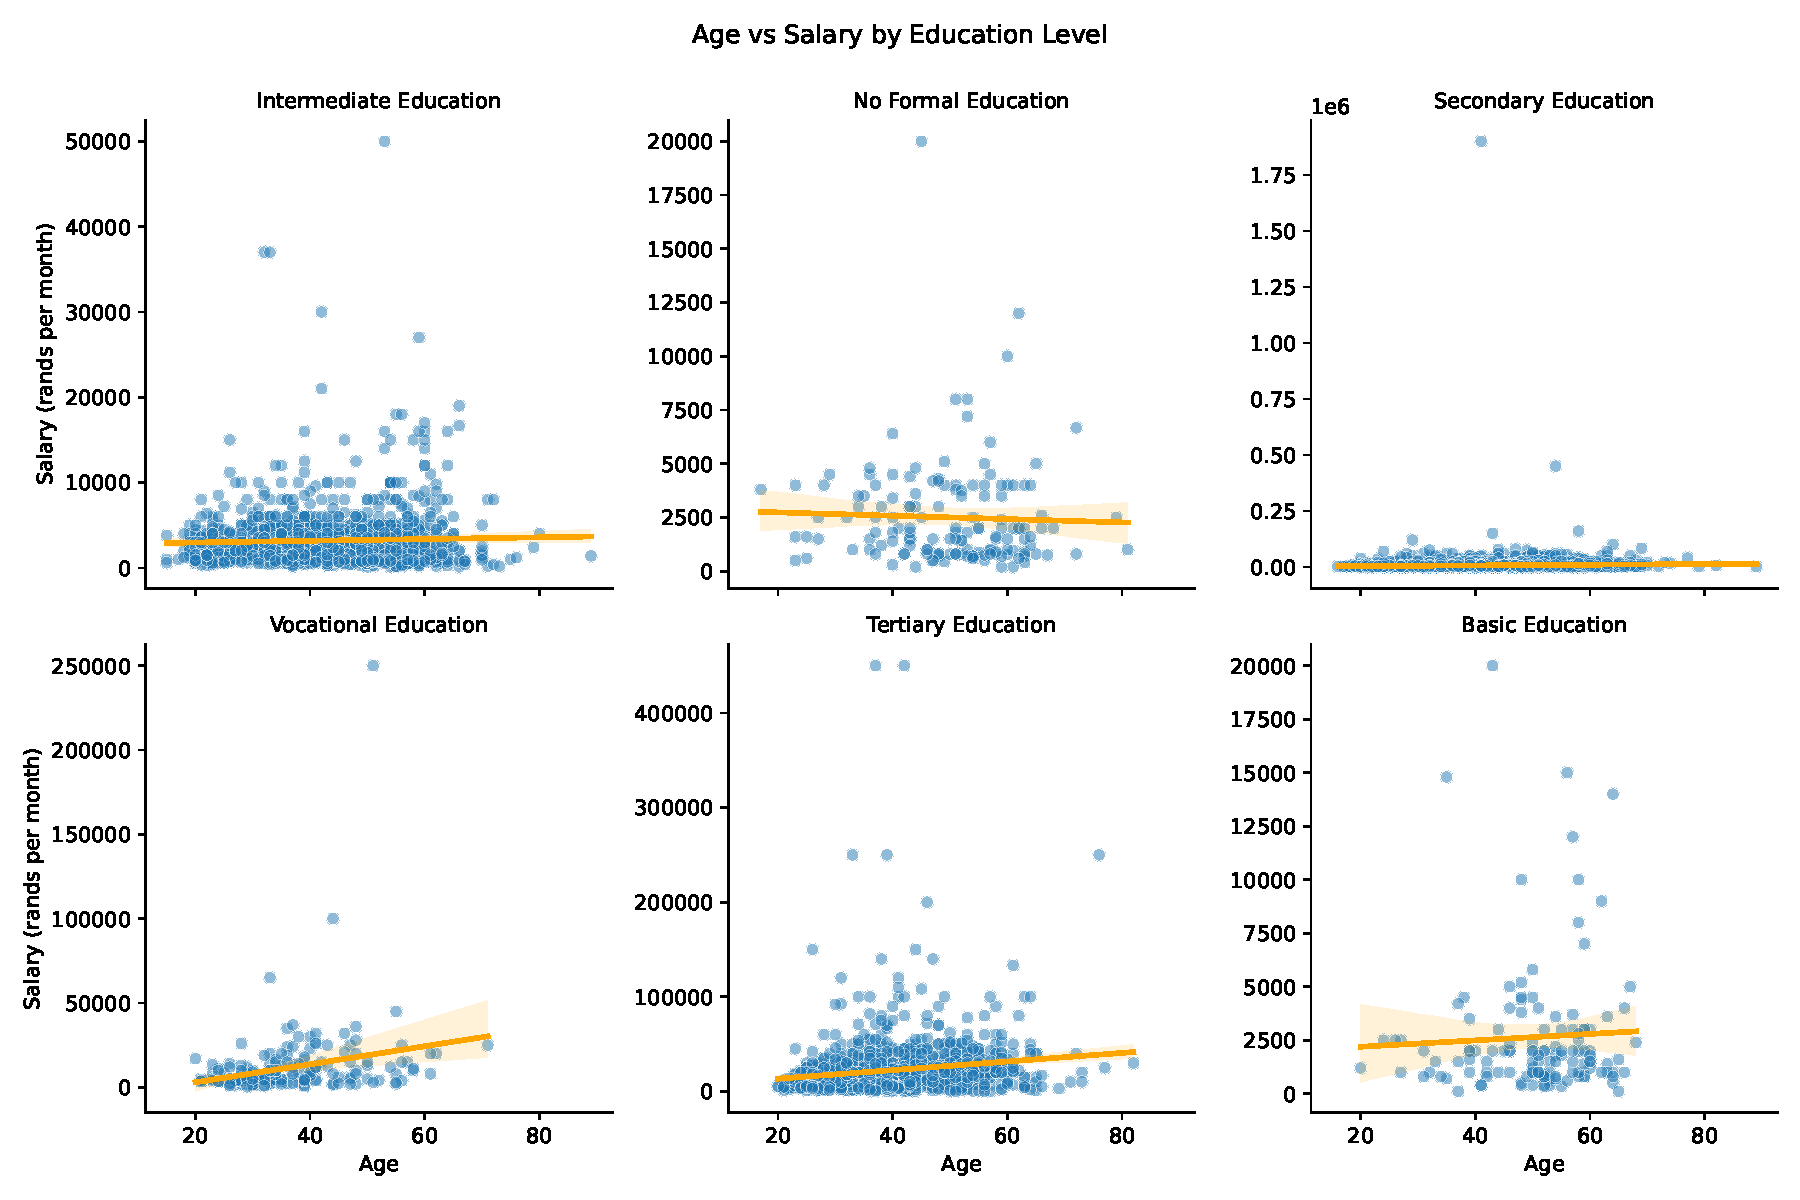
\includegraphics[width=\columnwidth]{images/hyp_3_facet.pdf} % Adjust the path accordingly
    \caption{Facet graph of salary distribution by age group}
    \label{fig:salary distribution facet}
\end{figure}

\subsubsection{Hypothesis 4: Gender and Salary/Education Level}

\begin{table}[H]
    \centering
    \caption{t-test results}
    \label{tab:t-test results}
    \begin{minipage}{\columnwidth}
        \input{data/hyp_4_t_test.tex}
    \end{minipage}
\end{table}

\begin{figure}[H]
    \centering
    \includegraphics[width=\columnwidth]{images/hyp_4_violin.pdf} % Adjust the path accordingly
    \caption{Violin plot of salary by gender}
    \label{fig:violin plot of salary by gender}
\end{figure}

\begin{figure}[H]
    \centering
    \includegraphics[width=\columnwidth]{images/hyp_4_bar_plot.pdf} % Adjust the path accordingly
    \caption{Histogram of gender count per highest education level}
    \label{fig:histogram of gender by education level}
\end{figure}

\begin{figure}[H]
    \centering
    \includegraphics[width=\columnwidth]{images/hyp_4_kde_plot.pdf} % Adjust the path accordingly
    \caption{Frequency of gender per salary}
    \label{fig:frequency of gender per salary}
\end{figure}

\subsubsection{Hypothesis 5: Ethnicity and Salary}

\begin{table}[H]
    \centering
    \caption{Anova test results}
    \label{tab:anova results}
    \begin{minipage}{\columnwidth}
        \input{data/hyp_5_anova.tex}
    \end{minipage}
\end{table}

\begin{figure}[H]
    \centering
    \includegraphics[width=\columnwidth]{images/hyp_5_violin_plot.pdf} % Adjust the path accordingly
    \caption{Violin plot of salary distribution by ethnicity}
    \label{fig:violin plot of salary distribution by ethnicity}
\end{figure}

\begin{table}[H]
    \centering
    \caption{Anova lm test results}
    \label{tab:anova lm results}
    \begin{minipage}{\columnwidth}
        \input{data/hyp_5_anova_lm.tex}
    \end{minipage}
\end{table}

\subsection{Clustering}

\subsubsection{K-Means Clustering}

\begin{figure}[H]
    \centering
    \includegraphics[width=\columnwidth]{images/clustering_k_means_inertia.pdf} % Adjust the path accordingly
    \caption{Inertia of K means clustering}
    \label{fig:inertia of k means clustering}
\end{figure}

\begin{figure}[H]
    \centering
    \includegraphics[width=\columnwidth]{images/clustering_k_means_sil.pdf} % Adjust the path accordingly
    \caption{Silhouette score of K meens clustering}
    \label{fig:silhouette of k means clustering}
\end{figure}

\begin{figure}[H]
    \centering
    \includegraphics[width=\columnwidth]{images/clustering_k_means.pdf} % Adjust the path accordingly
    \caption{K-Means clustering of age and salary}
    \label{fig:kMeans clustering of age and salary}
\end{figure}

\subsubsection{Hierarchical Clustering}

\begin{figure}[H]
    \centering
    \includegraphics[width=\columnwidth]{images/clustering_dendrogram.pdf} % Adjust the path accordingly
    \caption{Hierachical cluster dendrogram of income data}
    \label{fig:Hierachical cluster dendrogram of income data}
\end{figure}

\begin{figure}[H]
    \centering
    \includegraphics[width=\columnwidth]{images/clustering_dendro_sil.pdf} % Adjust the path accordingly
    \caption{Silhouette score for Hierachical cluster}
    \label{fig:Hierachical cluster silhouette score}
\end{figure}